\chapter{Introduction: What DB Researchers Prove, and How}
\setcounter{section}{-1}   % sections start at 0.0 (see main.tex comment)
\label{ch:intro}

\section{What these notes are}
These lecture notes are a \emph{toolbox tour} of the theoretical machinery that database
researchers actually use, extracted mechanically from the complete proceedings of
\textbf{SIGMOD~2026}: 385 research papers (PACMMOD Vol.~4, rounds 3--4, plus Vol.~3
issues 4--6, rounds 1--2). Every paper was fetched (arXiv \TeX{} sources when available,
ACM camera-ready PDFs otherwise), machine-extracted into formal statements, proofs, and
bound sentences (2{,}405 statements, 1{,}130 proofs), and 228 theory-relevant papers were
tagged with a controlled vocabulary of properties, tools, domains, and roles. The
aggregates behind every figure in this chapter come from that survey; every worked example
in the later chapters is a real paper from the corpus, cited in that chapter's reference
list.

Two honesty markers used throughout:
\begin{itemize}
\item \pods\ marks exemplars from the \textbf{PODS'26 issue} (PACMMOD Vol.~4 No.~2, DOI
  band 10.1145/3801890--3801919): 29 of the 228 tagged papers (12.7\%). They are part of
  the proceedings bundle; they often provide particularly clean exhibits of a tool, but
  they carry the theory-first culture of a sibling conference.
\item Formal statements are transcribed from machine extraction of the papers; where the
  extraction was noisy we paraphrase conservatively rather than decorate.
\end{itemize}

\section{The survey questions}
\begin{enumerate}
\item \textbf{Modeling} --- how do papers formalize a systems problem (cost model,
  adversary, noise model, distance metric)?
\item \textbf{Properties} --- what do they prove about the artifact: correctness,
  complexity bounds, approximation/competitive ratios, statistical guarantees?
\item \textbf{Tools} --- which theoretical machinery delivers the proof?
\item \textbf{Role} --- does theory motivate the work, drive the design, serve as the
  evaluation yardstick, or \emph{is} it the contribution?
\end{enumerate}

\section{Properties: first correct, then fast}
Figure~\ref{fig:props-tools} (left) ranks what the 228 tagged papers prove. The headline
surprise of the full-corpus count: \textbf{correctness is \#1} (98 papers, 43\%) --- ahead of
upper bounds (75) and probabilistic guarantees (42). The typical SIGMOD theory section is
not a big theorem; it is a small invariant certifying that a component preserves a
property (monotonicity of timestamps, order-independence of index construction,
merge-safety of compressed blocks). Hardness (36) plays a different role: the standard
\emph{license for heuristics} in graph search, repair, and mining papers. The tail is
where culture lives: \textbf{tightness} (11 --- matching upper and lower bounds, a 5.5$\times$
jump over the arXiv-only view of the corpus) and freshly activated slots such as
competitive ratio and regret bounds (2 papers each, entering through systems doors:
when to adapt, when to stop).

\section{Tools: a trinity plus a riser}
Figure~\ref{fig:props-tools} (right) ranks the machinery. A \emph{trinity} dominates:
\textbf{reductions} (52 papers), \textbf{concentration inequalities} (39), and
\textbf{induction} (37) --- respectively the tools of the hardness culture, the
statistical-certification culture, and the component-correctness culture. The big riser
once the ACM-only mass arrived is \textbf{exchange-greedy} (4$\to$17 papers): prove a
selection problem is a submodular/metric instance, inherit the approximation factor.
Chapter~\ref{ch:map} (the index table) maps each tool to its chapter.

\begin{widefigure}[htbp]
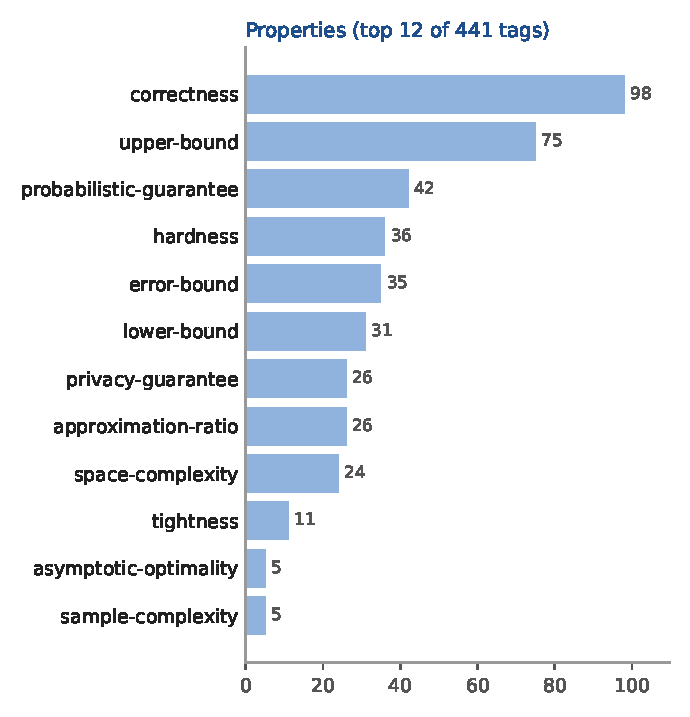
\includegraphics[width=.48\linewidth]{figures/f_props.pdf}\hfill
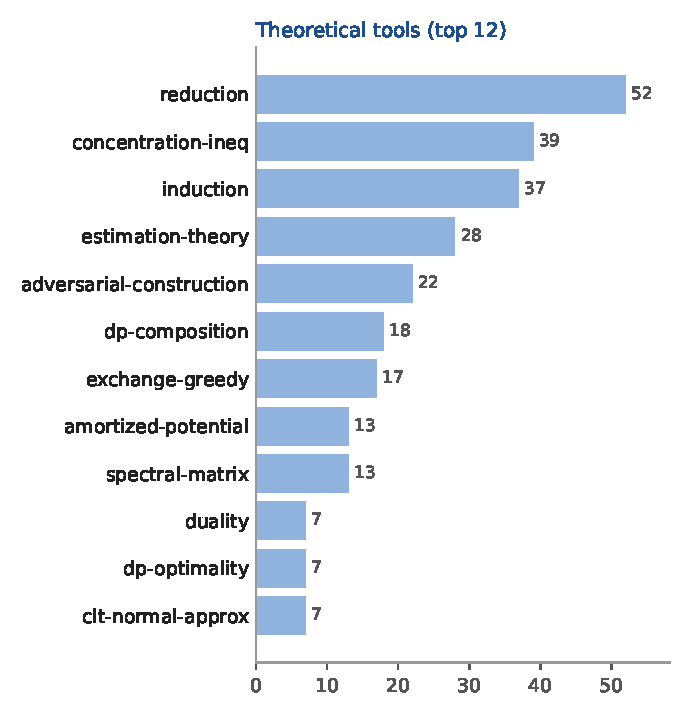
\includegraphics[width=.48\linewidth]{figures/f_tools.pdf}
\caption{Left: most-studied properties (top 12 of 441 property tags on the 228 tagged
papers). Right: most-used theoretical tools (top 12) --- each later chapter is one
tool.}\label{fig:props-tools}
\end{widefigure}

\section{Domains and dialects}
Figure~\ref{fig:domains-pairs} (left) shows where theory lives. Graph systems (56 papers)
are now the dominant dialect --- hardness $\to$ branch-and-bound and parameterized
algorithms $\to$ index-correctness lemmas. Privacy (26) is a near-monoculture of
composition accounting (69\% of its papers), increasingly in R\'enyi/f-DP currency.
Streaming and sketching splits into a pure-theory wing (matching lower bounds) and estimator
systems; vector search (25) splits between CLT-style certification and structural
correctness of graphs and routers.

\section{The playbook: property $\times$ tool pairings}
Figure~\ref{fig:domains-pairs} (right) is the survey's central cross-tab: which tool
delivers which property. The two workhorses are \textbf{hardness $\times$ reduction}
(32 papers) and \textbf{correctness $\times$ induction} (29). The pattern to
internalize: DB theory compresses into about eight such pairings, and each chapter of
these notes ends with the pairing(s) its tool owns.

\begin{widefigure}[htbp]
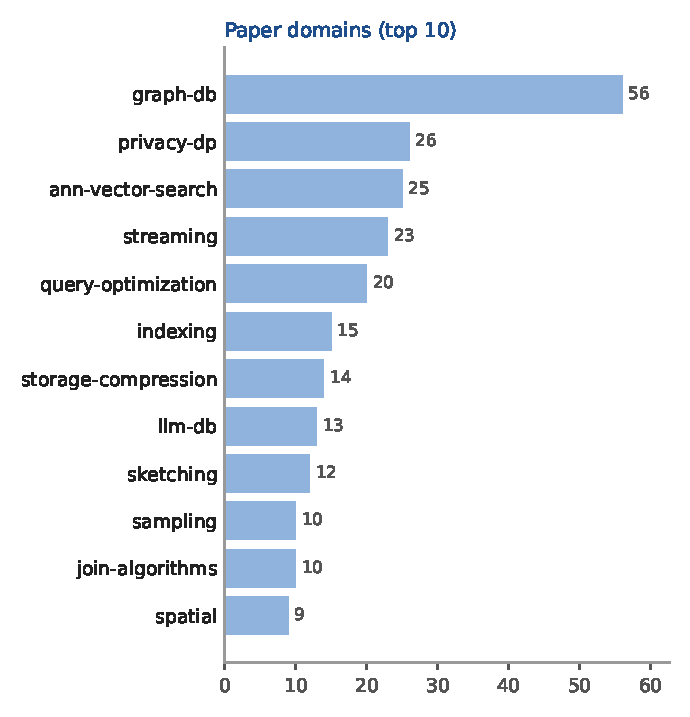
\includegraphics[width=.48\linewidth]{figures/f_domains.pdf}\hfill
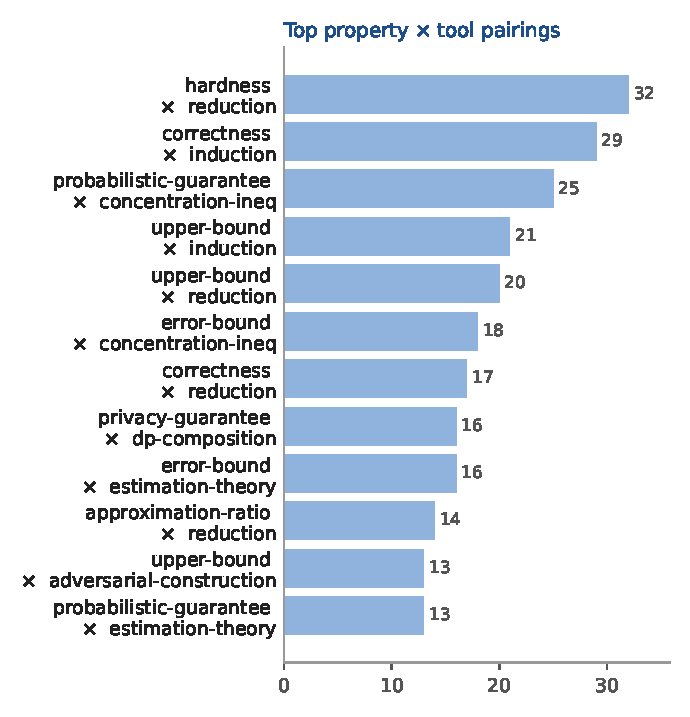
\includegraphics[width=.48\linewidth]{figures/f_pairs.pdf}
\caption{Left: paper domains (top 10). Right: top property$\times$tool pairings
(top 10) --- the ``playbook''.}\label{fig:domains-pairs}
\end{widefigure}

\section{Where theory sits}
66\% of tagged papers use theory as a \emph{design driver}; in 25\% the formal result
\emph{is} the paper (concentrated in the PODS issue and the pure streaming enclave);
motivation-only and evaluation-yardstick roles cover the rest. The role split matters
when reading exemplars: a design-driver paper proves what it builds; a
theory-as-contribution paper builds nothing and proves everything.

\section{Chapter map}
\label{ch:map}
Each of the following chapters is one tool: the formal core, then real SIGMOD~2026
exemplars with minimal context, then a ``when to reach for it'' box. Exemplars are
transcribed from the papers' own statements, with PODS-issue exemplars capped at one per
chapter (two for communication complexity, whose corpus presence is small); a paper may
recur in a second chapter when it is a clean exhibit of two tools --- each chapter
treats it under its own lens, and the \pods\ marker identifies PODS-issue exemplars in
the text.

\begin{widetable}[htbp]
\caption{Chapter map, ordered by how often the corpus uses each tool.
``Papers'' = tagged corpus papers using the tool; ``Ex.'' = exemplars
featured in the chapter.}
\label{tab:map}
\begin{tabular}{rllc}
\toprule
Ch. & Tool & Papers & Ex. \\
\midrule
1 & Reductions & 52 & 6 \\
2 & Concentration inequalities & 39 & 5 \\
3 & Induction & 37 & 6 \\
4 & Estimation theory & 28 & 6 \\
5 & Adversarial constructions & 22 & 6 \\
6 & DP composition & 18 & 6 \\
7 & Exchange--greedy arguments & 17 & 6 \\
8 & Spectral / matrix tools & 13 & 6 \\
9 & Amortized--potential analysis & 13 & 6 \\
10 & Coresets \& randomized NLA & 8 & 6 \\
11 & Information-theoretic bounds & 5 & 5 \\
12 & Communication complexity & 4 & 4 \\
13 & Online decisions (competitive \& regret) & 4 & 4 \\
\bottomrule
\end{tabular}
\end{widetable}

Tools not large enough for their own chapter in this corpus but worth knowing by name:
adversarial-adjacent duality/LP arguments (7 papers), dynamic programming optimality (7),
CLT/normal approximations (7), dyadic peeling (6), sketch mergeability theory (6),
balls-bins-hashing (5) --- several appear as guest stars inside the thirteen chapters.

\section{How these notes were made}
\label{sec:provenance}
The survey was scripted end to end: the 385-paper list came from OpenAlex, sources were
fetched (arXiv \TeX{} when available, ACM camera-ready PDFs otherwise), statements,
proofs, and bound sentences were machine-extracted (2{,}405 statements, 1{,}130 proofs),
and the 228 theory-relevant papers were tagged against the controlled vocabulary above;
every figure and count in this chapter is a direct aggregate of those tags.

These lecture notes are typeset with the \texttt{tufte-book} class of the
Tufte-\LaTeX{} project (Apache~2.0), as bundled in Boaz Barak's \texttt{panbook}
(MIT); the layout conventions --- margin-column learning objectives, themed remark and
recap blocks, end-of-proof markers, per-chapter references --- follow Barak's
\emph{Introduction to Theoretical Computer Science} notes (text licensed
CC~BY-NC-ND~4.0; we borrow the conventions only, no content). License notices for the
distributed class files ship with the sources.
